% Figure 4.4 (Session 4): the transverse-field Ising chain at zero, critical and large field.
% The image is rendered by figures/blender/s4_4_tfi.py; the coordinates of the labels come from
% figures/blender/out/tfi_anchors.tex. Compile with:
%   pdflatex tfi.tex ; result moves to ../mps_spin_chains/tfi.pdf
\documentclass[11pt,tikz,border=0pt]{standalone}
\usepackage{amsmath,amssymb,graphicx}
\usepackage{xcolor}
\definecolor{coursedark}{HTML}{1B2A4A}
\definecolor{costamber}{HTML}{B8620A}
\newlength{\figw}\setlength{\figw}{16.19cm}   % the text width of the notes (letter, 2.7 cm margins), so labels print at size
\newcommand{\ket}[1]{|#1\rangle}

\begin{document}
\begin{tikzpicture}[lbl/.style={font=\small, text=coursedark}]
  \node[anchor=south west, inner sep=0pt] at (0,0)
    {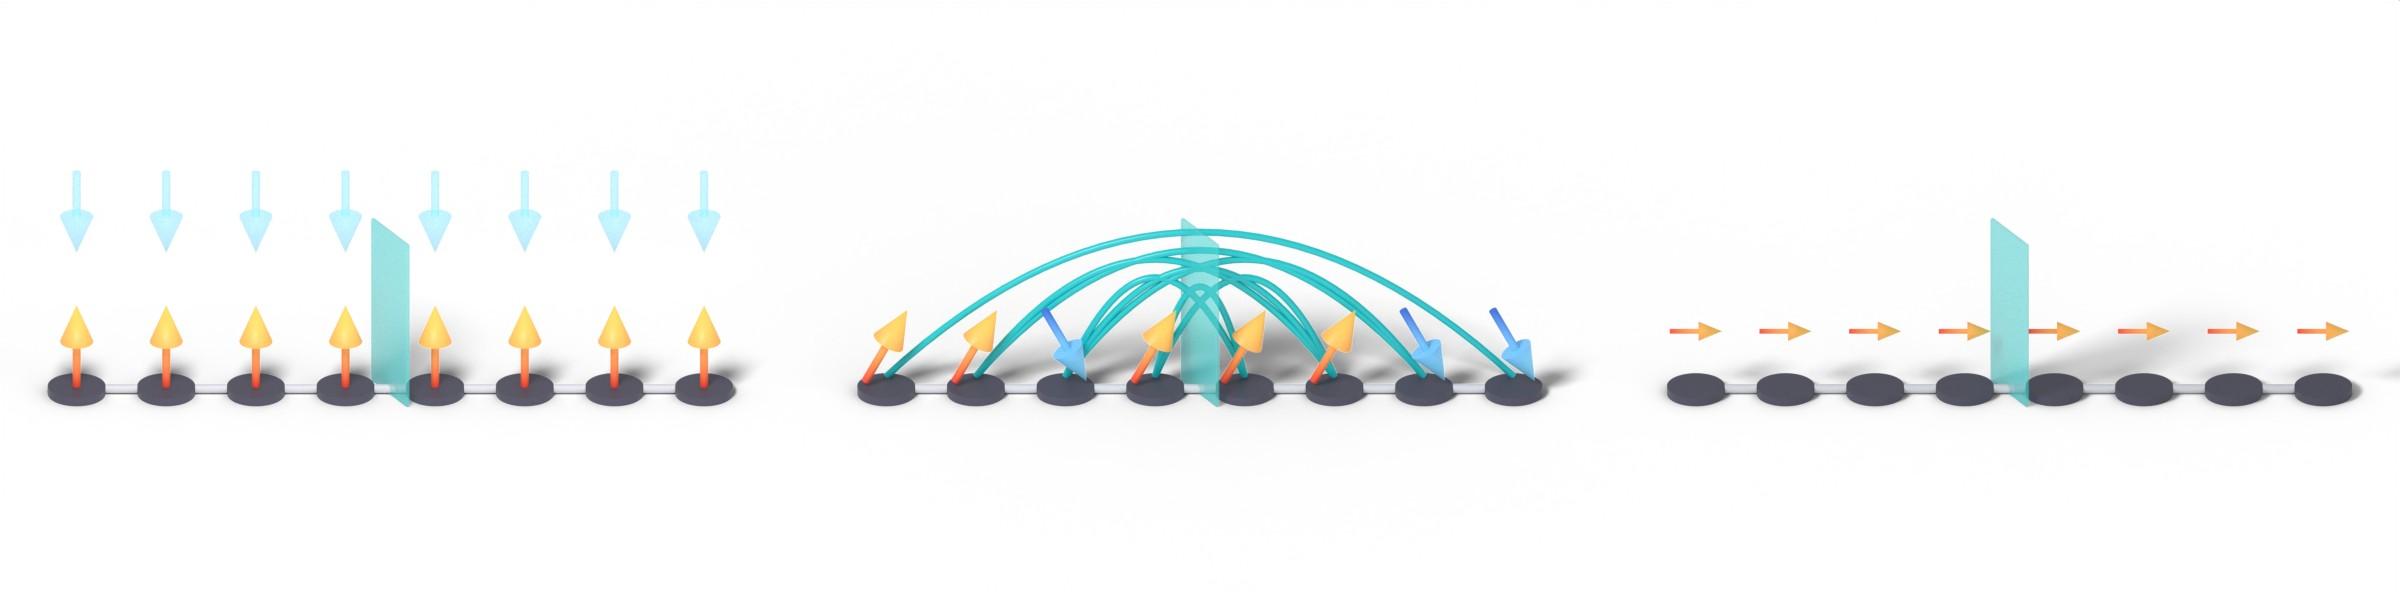
\includegraphics[width=\figw]{../blender/out/tfi.jpg}};
  %% written by figlib.py; x and y in units of the image width
\coordinate (ghost) at (0.1627\figw,0.1864\figw);
\coordinate (a) at (0.0048\figw,0.2240\figw);
\coordinate (lbla) at (0.1627\figw,0.0715\figw);
\coordinate (b) at (0.3422\figw,0.2240\figw);
\coordinate (lblb) at (0.5000\figw,0.0715\figw);
\coordinate (c) at (0.6795\figw,0.2240\figw);
\coordinate (lblc) at (0.8373\figw,0.0715\figw);

  \node[lbl, font=\normalsize, anchor=west] at (a) {(a)};
  \node[lbl, font=\normalsize, anchor=west] at (b) {(b)};
  \node[lbl, font=\normalsize, anchor=west] at (c) {(c)};
  \node[lbl, anchor=south] at (ghost) {partner $\lvert\downarrow\downarrow\cdots\downarrow\rangle$};
  \node[lbl, anchor=north] at (lbla) {$B_x=0$, \ $S_A=0$};
  \node[lbl, anchor=north] at (lblb) {$B_x\approx J/2$, \ $S_A$ largest};
  \node[lbl, anchor=north] at (lblc) {$B_x\gg J$, \ $S_A=0$};
\end{tikzpicture}
\end{document}
